\documentclass[10pt,twocolumn]{article}
\usepackage[T1]{fontenc}
\usepackage[utf8]{inputenc}
\usepackage{times}
\usepackage[margin=0.75in,columnsep=0.28in]{geometry}
\usepackage{microtype,booktabs,amsmath,amssymb,amsthm}
\usepackage[dvipsnames]{xcolor}
\usepackage{tikz}
\usetikzlibrary{arrows.meta,positioning,shapes.geometric}
\usepackage[hidelinks]{hyperref}
\usepackage{enumitem}
\setlist{nosep,leftmargin=1.2em}
\usepackage{titlesec}
\titlespacing*{\section}{0pt}{1.1ex}{0.6ex}
\titlespacing*{\subsection}{0pt}{0.8ex}{0.4ex}
\titleformat{\section}{\normalfont\large\bfseries}{\thesection}{0.5em}{}
\titleformat{\subsection}{\normalfont\normalsize\bfseries}{\thesubsection}{0.5em}{}
\usepackage{caption}
\captionsetup{font=small,labelfont=bf,skip=3pt}

\newtheorem{theorem}{Theorem}
\newcommand{\G}{\mathcal{G}}
\newcommand{\code}[1]{\texttt{\small #1}}
\definecolor{dk}{RGB}{20,60,120}
\definecolor{rd}{RGB}{170,30,30}
\definecolor{gn}{RGB}{20,110,50}
\newcommand{\thm}[1]{\textcolor{dk}{\textbf{#1}}}

\title{\vspace{-3ex}\textbf{SwarmGate: A Swarm Runtime with Lean-Verified Typed Messages}\\[0.3ex]
\large Turning a communication protocol into the security boundary of a multi-agent system}
\author{}
\date{}

\begin{document}
\twocolumn[
\maketitle
\vspace{-6ex}
\begin{quote}\small\itshape
\textbf{Abstract.} Large language model (LLM) agents cannot be type-checked: their behaviour is a
stochastic policy an attacker can steer through prompt injection, so no amount of checking an agent's
``program'' constrains what it does. Yet multi-agent systems fail precisely through \emph{communication}:
an injected agent infects its neighbours, a sub-agent talks a privileged agent into running code, an agent
skips a required approval, a swarm loops forever. We make the declared communication protocol the security
boundary. A small protocol language compiles to a finite automaton, and a \emph{reference monitor} mediates
every message, delivering it only if the protocol permits it at that point. Because the agents are
untrusted, the guarantee must come from the monitor---so we verify the monitor, in Lean 4. Our central
theorem states that for \emph{every} behaviour of \emph{every} agent, including a single adaptive adversary
controlling all of them, the delivered message trace stays within the protocol. The \emph{same} compiled
Lean function the theorems are about is the function the runtime runs. On top of enforcement we verify
blame assignment, transfer of past-time-temporal safety properties, an information-flow bound against
injection propagation, decentralised enforcement by per-role sidecars, and anti-runaway bounds---all with
no \code{sorry} and only Lean's standard axioms. Protocol enforcement provably secures the swarm's
\emph{control plane}; the \emph{data plane} of free text is bounded, not eliminated, and a verified
information-flow check flags unsafe designs before deployment. On a library of 20 real multi-agent
patterns, 78 generated theorems are re-checked by the Lean kernel; across $28{,}561$ scripted structural
attacks the monitor admits $0.0\%$ while delivering $100\%$ of honest traffic; and the runtime enforces any
framework, including real LLM agents, over A2A messages and MCP tool calls at microsecond cost.
\end{quote}
\vspace{1ex}
]

\section{The problem, and the idea}

A single LLM gets things wrong; a \emph{swarm} of them fails in new ways, and the new ways run through the
messages they exchange. \emph{Prompt Infection}~\cite{lee2024promptinfection} and infectious
jailbreaks~\cite{gu2024agentsmith} spread one compromise across the network. A fooled orchestrator will
hand malicious code to an executor~\cite{triedman2025mas}; an agent-in-the-middle rewrites traffic to
hijack a task~\cite{he2025aitm}. Empirically, a large fraction of multi-agent failures are
inter-agent coordination faults---skipped verification steps, premature termination, disobeyed role
specs---not single-model mistakes~\cite{cemri2025mast}, and the open problem of \emph{multi-agent
security} is now stated as such~\cite{schroederdewitt2025open,hammond2025multiagent}.

These are failures of \emph{communication structure}: who may talk to whom, in what order, carrying what.
Computer science has a precise tool for communication structure---\emph{multiparty session
types}~\cite{honda2008mpst,honda2016mpst}---which guarantee that a system of processes follows a global
protocol. But session types work by \emph{type-checking each participant's program}, and an LLM agent has
no program to check: it is a sampling procedure whose next message depends on a context an attacker may
have poisoned. The classical guarantee evaporates exactly when we need it.

\textbf{Our idea is to invert the trust relationship.} Keep the protocol; stop trusting the agents; and
obtain the guarantee from a \emph{runtime reference monitor}~\cite{schneider2000enforceable} that
completely mediates communication and rejects any message the protocol does not allow right now. The
monitor, not the agent, is what must be correct---so we \emph{verify the monitor} in Lean~4, and we run the
\emph{same} verified function we proved about. The protocol becomes an enforced security policy, and
``which messages are legal'' becomes a machine-checked property rather than a hope about model behaviour.

This single move organises everything that follows (Figure~\ref{fig:arch}). It draws a sharp and honest
line. The protocol governs the swarm's \textbf{control plane}---recipients, ordering, labels, payload
shapes, choices, recursion---and we \emph{provably} enforce it against arbitrary adversaries. It cannot by
itself govern the \textbf{data plane}, the free-text content of a message, because a well-typed
\code{string} can still hide an instruction. So we also make the control plane do as much data-plane work
as the types allow: narrow payload types (enums, bounded integers, refinements) that cannot carry an
injection, and a \emph{verified information-flow bound} that confines where untrusted text may travel. The
contribution is one coherent story---\emph{the protocol is the boundary, the monitor is verified, the
agents are free}---not a list of features.

\begin{figure}[t]
\centering
\resizebox{\columnwidth}{!}{%
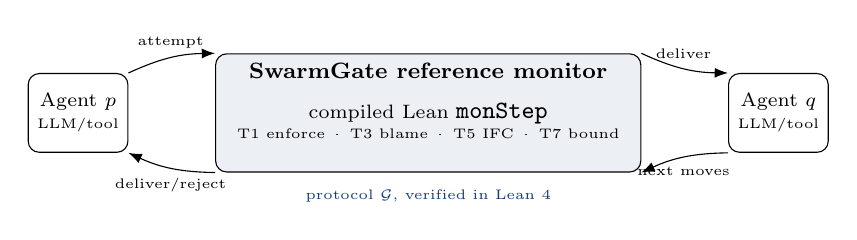
\begin{tikzpicture}[font=\scriptsize,node distance=3mm]
\node[draw,rounded corners,fill=dk!8,minimum width=5.4cm,minimum height=1.5cm] (g) {};
\node[anchor=north] at (g.north) {\footnotesize\textbf{SwarmGate reference monitor}};
\node[align=center] at ([yshift=-1mm]g.center) {compiled Lean \code{monStep}\\[-0.3ex]{\tiny T1 enforce \,·\, T3 blame \,·\, T5 IFC \,·\, T7 bound}};
\node[draw,rounded corners,fill=white,left=1.1cm of g,minimum height=1.0cm,align=center] (p) {Agent $p$\\{\tiny LLM/tool}};
\node[draw,rounded corners,fill=white,right=1.1cm of g,minimum height=1.0cm,align=center] (q) {Agent $q$\\{\tiny LLM/tool}};
\draw[-{Latex}] (p.north east) to[bend left=12] node[above,midway]{\tiny attempt} (g.north west);
\draw[-{Latex}] (g.south west) to[bend left=12] node[below,midway]{\tiny deliver/reject} (p.south east);
\draw[-{Latex}] (g.north east) to[bend right=12] node[above,midway]{\tiny deliver} (q.north west);
\draw[-{Latex}] (q.south west) to[bend right=12] node[below,midway]{\tiny next moves} (g.south east);
\node[below=1mm of g,font=\tiny,text=dk] {protocol $\G$, verified in Lean 4};
\end{tikzpicture}}
\caption{Agents communicate \emph{only} through the monitor. No agent holds a handle on another; every
message is an \emph{attempt} the monitor delivers or rejects. The decision is the compiled Lean function
the theorems are about.}
\label{fig:arch}
\vspace{-1ex}
\end{figure}

\section{Protocols as verified automata}

A protocol names a set of \emph{roles} and fixes how they interact. Roles may be LLM agents, tools, or
humans; a tool is just a role whose messages are calls and results. We write protocols in a small
Scribble-like language; the example in Figure~\ref{fig:dsl} says: the user gives the agent a task; then, for
at most five rounds, the agent proposes a command (an \code{enum} choice plus a short argument with no
shell metacharacters) to a \emph{human}, who either approves---after which the agent may call the shell and
loop or finish---or denies.

\begin{figure}[t]
\footnotesize
\begin{tabbing}
xx\=xx\=xx\=\kill
\code{protocol ApprovalGate \{}\\
\>\code{roles User, Agent, Human, Shell;}\\
\>\code{endorser Human;}\quad\textcolor{gn}{\tiny// non-LLM, can't be injected}\\
\>\code{sensitive Agent -> Shell;}\\[0.3ex]
\>\code{User -> Agent : Task(str) where len <= 2000;}\\
\>\code{rec Step max 5 \{}\quad\textcolor{gn}{\tiny// bounded: no runaway loop}\\
\>\>\code{Agent -> Human : Propose(\{cmd: enum\{ls,cat,df\},}\\
\>\>\quad\code{arg: str\}) where arg.len<=120 and arg !contains ";";}\\
\>\>\code{choice at Human \{}\\
\>\>\>\code{Human -> Agent : Approve(...);}\\
\>\>\>\code{call Agent -> Shell : exec(...) returns str;}\\
\>\>\>\code{choice at Agent \{ continue Step; \}}\\
\>\>\>\quad\code{or \{ Agent -> User : Done(str); \} }\\
\>\>\code{\} or \{ Human -> Agent : Deny(str); ... \} \}}\\
\>\code{property NoUnapprovedExec:}\\
\>\quad\code{Agent->Shell:exec implies prev Human->Agent:Approve;}\\
\code{\}}
\end{tabbing}
\vspace{-1.5ex}
\caption{A protocol in the SwarmGate language. The meaning is the automaton it compiles to; the text is
only notation and is not trusted.}
\label{fig:dsl}
\vspace{-1.5ex}
\end{figure}

The meaning of a protocol is the finite \emph{guarded automaton} it compiles to: states, and transitions
\(p \!\to\! q : \ell(S)\{\varphi\}\) labelled by sender, recipient, message label~$\ell$, a payload
type~$S$ and a decidable refinement~$\varphi$ (e.g.\ \code{len <= 120}). A concrete event
\(p \!\to\! q : \ell(v)\) \emph{matches} a transition when the endpoints and label agree and the value~$v$
has type~$S$ and satisfies~$\varphi$. The executable one-step function \code{step} takes the first matching
transition; folding it over a trace gives the \emph{prefix language}~$\mathrm{Pref}(\G)$, which is
prefix-closed---a safety property in the sense of Alpern--Schneider, and exactly what a monitor can enforce.
Working with automata rather than recursive session types keeps every check decidable and sidesteps
coinduction, following recent automata-based treatments of
implementability~\cite{li2023complete,castroperez2026synthetic}. We prove the executable semantics
coincides with a relational specification, so later theorems about \code{step} are theorems about the
declarative protocol.

\section{What we prove}

All definitions and proofs are in Lean~4 (\(\sim\)2{,}200 lines), depend only on
\code{propext}, \code{Classical.choice}, \code{Quot.sound}, and contain no \code{sorry}. We summarise the
results as one narrative; the bold names are the Lean theorems.

\subsection{Enforcement: the agents are free, the trace is not}

The monitor keeps a protocol state, a delivered-message count, a per-role strike counter and a kill
switch. One step is the function in Figure~\ref{fig:step}: it authenticates the sender against the claimed
source role, checks quarantine, budget, and whether the event matches an enabled transition, and either
delivers (advancing the state) or rejects with a blamed principal and a reason. An \emph{adversary} is
\emph{any} function from the history of past verdicts to the next attempted message; quantifying over all
finite attempt lists subsumes every adversary, including one that has compromised all agents at once and
adapts to each decision.

\begin{figure}[t]
\footnotesize\setlength{\fboxsep}{4pt}
\fbox{\parbox{0.93\columnwidth}{\ttfamily\scriptsize
monStep cfg P m (send $\sigma$ e) =\\
\hspace*{1em}\textbf{if} m.halted\hspace{3.0em}$\Rightarrow$ reject $\sigma$ halted\\
\hspace*{1em}\textbf{elif} quarantined cfg m $\sigma$\hspace{0.4em}$\Rightarrow$ reject $\sigma$ quarantined\\
\hspace*{1em}\textbf{elif} $\sigma \neq$ e.src\hspace{3.2em}$\Rightarrow$ strike; reject $\sigma$ spoof\\
\hspace*{1em}\textbf{elif} m.count $\geq$ budget\hspace{1.2em}$\Rightarrow$ reject $\sigma$ budget\\
\hspace*{1em}\textbf{else match} step P m.s e \textbf{with}\\
\hspace*{2em}| some s' $\Rightarrow$ \{m.s:=s', count+1\}; \textbf{deliver} e\\
\hspace*{2em}| none\hspace{1.2em}$\Rightarrow$ strike; reject $\sigma$ notEnabled
}}
\vspace{-1ex}
\caption{The gate, verbatim from \code{Monitor.lean} (simplified). Theorems T1--T3$'$ are about \emph{this}
function, and the runtime executes its compiled form.}
\label{fig:step}
\vspace{-1.5ex}
\end{figure}

\begin{theorem}[Enforcement, \thm{enforcement}/\thm{enforcement\_adaptive}]
For every protocol~$\G$ and every sequence of attempts, the sequence of delivered messages is a run of~$\G$
from its start state; hence it lies in $\mathrm{Pref}(\G)$. The same holds for every adaptive adversary and
every horizon.
\end{theorem}

\noindent This is the load-bearing result: \emph{a compromised agent cannot make the swarm step outside its
protocol.} Topology violations (messaging a non-neighbour, as in worm spread), out-of-order actions
(executing before approval), forged labels, role impersonation (an agent-in-the-middle position), ill-typed
or out-of-range payloads, and replay are all excluded, because none of them matches an enabled transition.
Two companion results make the monitor usable rather than merely safe. \thm{transparency}: conformant,
in-budget traffic is delivered unchanged---no false positives for honest agents. \thm{blame\_sound} and
\thm{honest\_never\_blamed}: a rejection always names the actual deviating sender, and an agent that only
ever sends authentic enabled messages is never blamed or quarantined, whatever the others do. Containment
results bound the damage of a compromise directly: once quarantined (\thm{quarantine\_contains}) or after
the kill switch (\thm{kill\_contains}), nothing attributed to a principal is delivered again, and no run
ever delivers more than its budget (\thm{budget\_bound}).

\subsection{From protocol properties to runtime guarantees}

Enforcement says runs stay in the protocol; we also want to prove things \emph{about} the protocol and have
them hold at runtime for free. We support past-time linear temporal logic over events---\emph{``no shell
command unless a human approved earlier''} is \(H(\mathit{exec}\to O\,\mathit{approve})\). An incremental
monitor stores one bit per subformula; we prove it matches the recursive semantics, and then:

\begin{theorem}[Property transfer, \thm{property\_transfer}]
If the verified checker accepts a certificate for a past-time formula~$\psi$ on~$\G$, then on every enforced
run---whatever the agents do---$\psi$ holds after every delivered event.
\end{theorem}

The checker uses \emph{translation validation}: unverified exploration produces a candidate invariant set
over (protocol state, monitor bits); a small verified checker confirms it contains the initial
configuration, satisfies the invariant, and is closed under successors; and one generic lemma turns that
into coverage of all reachable configurations. Each protocol thus earns a machine-checked guarantee without
re-proving meta-theory, and when a property \emph{fails} the explorer returns the shortest violating trace.
The same certificate machinery yields the anti-runaway results---\emph{no stuck state}
(\thm{no\_stuck}: every reachable non-final state has a legal move, so honest agents never dead-end),
\emph{completion always reachable} (\thm{completion\_possible}), and \emph{bounded runs}
(\thm{bounded\_length}: a bounded protocol delivers at most a fixed number of messages regardless of the
runtime budget).

\subsection{The data plane: an information-flow bound}

Enforcement secures the control plane completely, but a protocol that lets an agent send a free-text
\code{Notes(str)} it derived from a web page has handed the attacker a channel. An LLM cannot separate data
from instructions in its context, so \emph{taint is sticky per agent}: once a role receives high-capacity
content from a tainted source, everything it later sends is tainted. We label untrusted source roles, mark
some messages as low-capacity (an \code{enum} or bounded integer cannot carry a paragraph of injected
instructions), designate \emph{endorser} roles (humans, deterministic validators) that cannot be injected,
and mark the sensitive actions.

\begin{theorem}[Information flow, \thm{ifc\_transfer}]
If the verified checker accepts, then on every enforced run every delivered sensitive action is taken by a
role that never received high-capacity content derived from an untrusted source.
\end{theorem}

\noindent This is the protocol-level form of the dual-LLM / plan-then-execute / quarantined-reader
patterns~\cite{beurerkellner2025designpatterns,debenedetti2025camel}: the check \emph{proves} that a given protocol
actually implements the pattern, and when it does not it returns the taint path. Low-capacity typing also
gives a quantitative handle---the number of attacker-chosen bits that can reach a clean agent is bounded by
the capacities of the tainted$\to$clean edges on a run, which our analyser reports---connecting to the
collusion-bandwidth concern of the multi-agent-security
agenda~\cite{schroederdewitt2025open,hammond2025multiagent}.

\subsection{Decentralised enforcement}

A single trusted router is wrong for mutually distrusting organisations. By projecting the global protocol
onto each role we obtain per-role local automata that an organisation can enforce with its own sidecar; a
message is delivered when both endpoints' sidecars accept it. Projection is unverified, but we validate its
output:

\begin{theorem}[Decentralised soundness, \thm{decentralised\_sound}]
If the verified checker accepts the projection certificate, then every trace the sidecars jointly admit is
a trace of the global protocol; consequently property transfer and the information-flow bound hold with no
central router.
\end{theorem}

When a protocol is not implementable this way the checker returns the offending interleaving (a classical
realisability witness~\cite{alur2005realizability,li2023complete}), and the protocol must run centrally.

\subsection{The proof is the program}

Crucially, the runtime does not re-implement the monitor: its accept/reject decision is the compiled Lean
\code{monStep} the theorems quantify over, exposed as a JSON-lines server. For maximum assurance,
\code{swarmgate emit-lean} turns any protocol's certificates into a self-contained Lean file whose theorems
the \emph{kernel} re-checks---closing the specification-to-implementation gap that extraction-based
pipelines~\cite{castroperez2021zooid} and hand-written correspondences close less directly.

\section{Runtime and ecosystem}

A protocol is useful only if real swarms can run under it. The Python runtime executes agents that
communicate \emph{only} through a gate; an agent is activated by an incoming message, may attempt any
number of sends during its turn, and never obtains a reference to another agent. LLM agents use the
protocol as their tool interface: an agent's legal next moves become typed tools and every tool result
reports which moves are now allowed (``protocol-guided decoding''), so guidance and enforcement are
separable and separately measurable. Because enforcement lives at the message boundary, SwarmGate is
framework-agnostic: a \textbf{gateway} exposes the monitor as a network service for \emph{agent-to-agent}
(A2A-style) messaging and \emph{MCP} tool calls, so agents in any language participate by speaking
HTTP\,+\,JSON, and an MCP proxy restricts each agent to the tools its protocol permits in the current
state---least-privilege-per-step~\cite{sikaroudi2026concordat} driven by a multiparty protocol and usable
across a whole swarm.

\section{Evaluation}

We ask five questions.

\textbf{(E1--E2) Does it express real patterns, and does the kernel believe the proofs?} We encoded 20
widely used multi-agent patterns---supervisor/worker map-reduce, plan-and-execute, ReAct tool loops,
human-approval gates, debate, critic/reviser, two-phase commit, 2-of-2-approval payments, AutoGen-style
group chat, handoff routing, dual-LLM, cross-org procurement, and more. All 20 verify; \code{emit-lean}
produces 78 theorems that the Lean kernel re-checks in $\sim$62\,s total (median per-protocol check
52\,ms; largest automaton 30 states). Four protocols \emph{fail} the information-flow check by design---and
the tool returns the exact attack path---illustrating that the check discriminates safe from unsafe
designs; one protocol is reported \emph{unrealisable} decentrally with a witness.

\textbf{(E3) Does enforcement stop attacks a weaker defence misses?} We compare an ablation lattice of
gates, each adding one dimension of checking: none; payload-schema only (the guarantee a structured-output
or A2A message schema gives); a static topology ACL (who-may-talk-to-whom, as in agent-graph frameworks);
and the full session monitor (Python mirror and verified Lean binary). Against $28{,}561$ scripted
structural attacks in eight classes drawn from the literature (lateral movement, approval bypass,
impersonation, choice hijacking, payload smuggling, refinement violation, replay, runaway), Table~\ref{tab:struct}
shows the session monitor admits $0.0\%$ while all gates deliver $100\%$ of honest messages---and a static
topology ACL still admits a third of the attacks, because it ignores \emph{state}.

\begin{table}[t]\centering\small
\caption{Fraction of structural attacks \emph{admitted} (lower is better). Honest traffic delivered:
$100\%$ for every gate.}
\label{tab:struct}
\begin{tabular}{lrrrr}
\toprule
attack class & none & schema & topology & \textbf{session} \\
\midrule
wrong recipient      & 100 & 99.9 & 5.4 & \textbf{0.0}\\
out-of-order         & 100 & 100  & 100 & \textbf{0.0}\\
impersonation        & 100 & 100  & 0.0 & \textbf{0.0}\\
choice hijack        & 100 & 100  & 4.0 & \textbf{0.0}\\
ill-typed payload    & 100 & 0.0  & 0.0 & \textbf{0.0}\\
refinement violation & 100 & 0.0  & 0.0 & \textbf{0.0}\\
replay               & 100 & 100  & 100 & \textbf{0.0}\\
runaway              & 100 & 100  & 100 & \textbf{0.0}\\
\midrule
\textbf{all} (28{,}561) & 100 & 81.4 & 35.0 & \textbf{0.0}\\
\bottomrule
\end{tabular}
\vspace{-1ex}
\end{table}

\textbf{The control/data-plane split, made concrete.} In an ``ops swarm'' scenario (planner, researcher and
executor agents; web, shell and mail tools; an approver) we replace every agent with a worst-case
\emph{compromised} script that obeys any injection it actually receives. Against the \emph{naive} protocol,
weak gates let the attacker both run a rogue command and exfiltrate data (100\%). The session monitor stops
the control-plane hijack completely ($0\%$ rogue commands: the executor never accepts a command from
anyone but the endorsing approver), but a \emph{patient} attacker still exfiltrates through the protocol's
free-text mail body (80\%)---and this is exactly the protocol our information-flow check \emph{rejects at
design time}. The \emph{hardened} protocol, which \emph{passes} the check, stops both attacks at $0\%$
across every gate, because the planner never becomes tainted and the executor only accepts \code{enum}
commands. The lesson is the thesis in miniature (Table~\ref{tab:scenario}): enforcement secures the control
plane outright; the data plane is secured by \emph{designing} the protocol so the verified IFC check passes.

\begin{table}[t]\centering\small
\caption{Ops scenario, worst-case compromised agents: fraction of runs achieving each attack goal (lower is
better), averaged over five injection styles. ``ctrl'' = rogue command / lateral movement; ``data'' =
patient exfiltration through a free-text field. The IFC check \emph{rejects} the naive protocol and
\emph{accepts} the hardened one.}
\label{tab:scenario}
\begin{tabular}{llrr}
\toprule
protocol & gate & ctrl-plane & data-plane \\
\midrule
naive (IFC \textcolor{rd}{fails})   & none            & 100 & 100 \\
naive (IFC \textcolor{rd}{fails})   & \textbf{session} & \textbf{0} & 80 \\
hardened (IFC \textcolor{gn}{ok})   & none            & 0 & 0 \\
hardened (IFC \textcolor{gn}{ok})   & \textbf{session} & \textbf{0} & \textbf{0} \\
\bottomrule
\end{tabular}
\vspace{-1.5ex}
\end{table}

\textbf{(E4) Does it hold up with real LLMs?} Using real Claude agents in the same scenario with
injection-bearing web pages, we measure attack success with and without the monitor and benign-task
completion and false-reject rates. The harness (\code{eval/e4\_llm.py}) reports per-run cost; results are
included in the artifact.\footnote{The real-LLM study runs against the Anthropic API; numbers are in the
repository's \code{eval/results/llm.json} when an API key is configured.}

\textbf{(E5--E6) Overhead and faithfulness.} A monitor decision costs $0.64\,\mu$s in the Python mirror and
$\sim$68\,$\mu$s through the verified Lean binary (dominated by the pipe round-trip), both negligible
beside a multi-second LLM call; verification is tens of milliseconds and scales gently (115\,ms at 128
states). To be sure the convenient Python gate matches the verified one, we differential-test them on
$\sim$300{,}000 adversarial attempts across hundreds of random protocols: zero disagreements.

\section{Related work and position}

Session types and their mechanisation are a mature field: multiparty session
types~\cite{honda2008mpst,honda2016mpst,scalas2019less}, mechanised metatheory and certified processes in
Coq~\cite{castroperez2021zooid,tirore2023sound,keskin2026liveness} and
Lean~\cite{qin2026mech}, runtime monitoring of session types~\cite{bocchi2017monitoring,larsen2026nest},
blame~\cite{jia2016blame}, and the enforceability theory that says a safety property is exactly what an
execution monitor can guarantee~\cite{schneider2000enforceable,ligatti2005edit}. Applying protocol
discipline to LLM agents is very recent and concurrent: message-sequence-chart workflows with Lean-verified
deadlock-freedom~\cite{bollig2026provable}, single-agent typestate enforced by tool
masking~\cite{sikaroudi2026concordat}, choreographies~\cite{gopinathan2026pact}, and BSPL
enactment~\cite{joshi2026ahoy}; on the security side, permitted-control-flow enforcement for multi-agent
systems~\cite{triedman2025mas} and information-flow defences against prompt
injection~\cite{debenedetti2025camel,beurerkellner2025designpatterns}.

SwarmGate's position is the combination none of these occupies. Prior agent-protocol work aims at
\emph{coordination correctness assuming cooperative agents}; we treat the protocol as a \emph{security
policy enforced by a verified reference monitor against agents that may be fully compromised}, and we state
and mechanise that as our central theorem. Relative to the agent-protocol line we add multiparty payload
refinements checked at runtime, a verified information-flow bound against injection propagation, verified
blame and decentralised enforcement, and an evaluation against the known multi-agent attack classes.
Relative to the session-type line we move the principals from typed programs to arbitrary adversaries and
make the \emph{monitor} the proof obligation, run the verified definitions \emph{as} the runtime, and
target LLM swarms over A2A and MCP.

\section{Limitations}

We are deliberate about scope. SwarmGate does not judge the \emph{content} of a well-typed free-text
field---a \code{string} can hide an instruction; we bound where it flows, not what it means. It does not
make an agent's \emph{choices} correct---a compromised approver can legitimately approve, which is why
protocols should encode separation of duty (our payments protocol requires two approvers) and k-of-n
checks. It proves the monitor matches the specification and the specification has the stated properties,
not that the specification is the \emph{right} policy. And it assumes complete mediation and authenticated
senders; attacks outside the mediated channel---tool poisoning, model backdoors, shared-memory
side-channels---need orthogonal defences. Within its boundary, though, the guarantee is unconditional: no
behaviour of any agent moves the swarm outside its protocol, and that is now a theorem.

{\footnotesize
\bibliographystyle{abbrv}
\bibliography{refs}
}

\end{document}
